\documentclass[40pt]{article}
\usepackage{ctex}
\usepackage{CJK}
\usepackage{graphicx}
\usepackage{picinpar,graphicx}
\usepackage{cite}
\usepackage{multirow}
\usepackage{hyperref,amsmath,amssymb,amscd}
\usepackage{geometry}
\setmainfont{Times New Roman}
\geometry{left=0.3cm,right=0.5cm,top=2.5cm,bottom=2.5cm}%Maybe it is the right choice.....
\usepackage{setspace}
\setlength{\parindent}{2em}
\twocolumn
\begin{document}
\title{\textbf{Reverse Connection with Objectness Prior Networks for Object Detection IV}}
\author{\textbf{Liangjie Cao}}
\date{\textbf{23 May 2018}}
\maketitle
\par
\setlength{\baselineskip}{15pt}
\section{Training and Testing results}
\textbf{Finally they train and evaluate our models on three major datasets: PASCAL VOC 2007, PASCAL VOC 2012, and MS COCO. For fair comparison, all experiments are based on the VGG-16 networks. We train all our models on a single Nvidia TitanX GPU, and demonstrate state-of-the-art results on all three datasets.  As shown in Table~\ref{Table1}, all methods have inferior performance on ‘boat’ and ‘bottle’. However, RON improves performance of these categories by significant margins: 4.0 points improvement for ‘boat’ and 7.1 points improvement for ‘bottle’. In summary, performance of 17 out of 20 categories has been improved by RON.~\ref{Figure1}}
\begin{figure}[htbp]
 \centering
 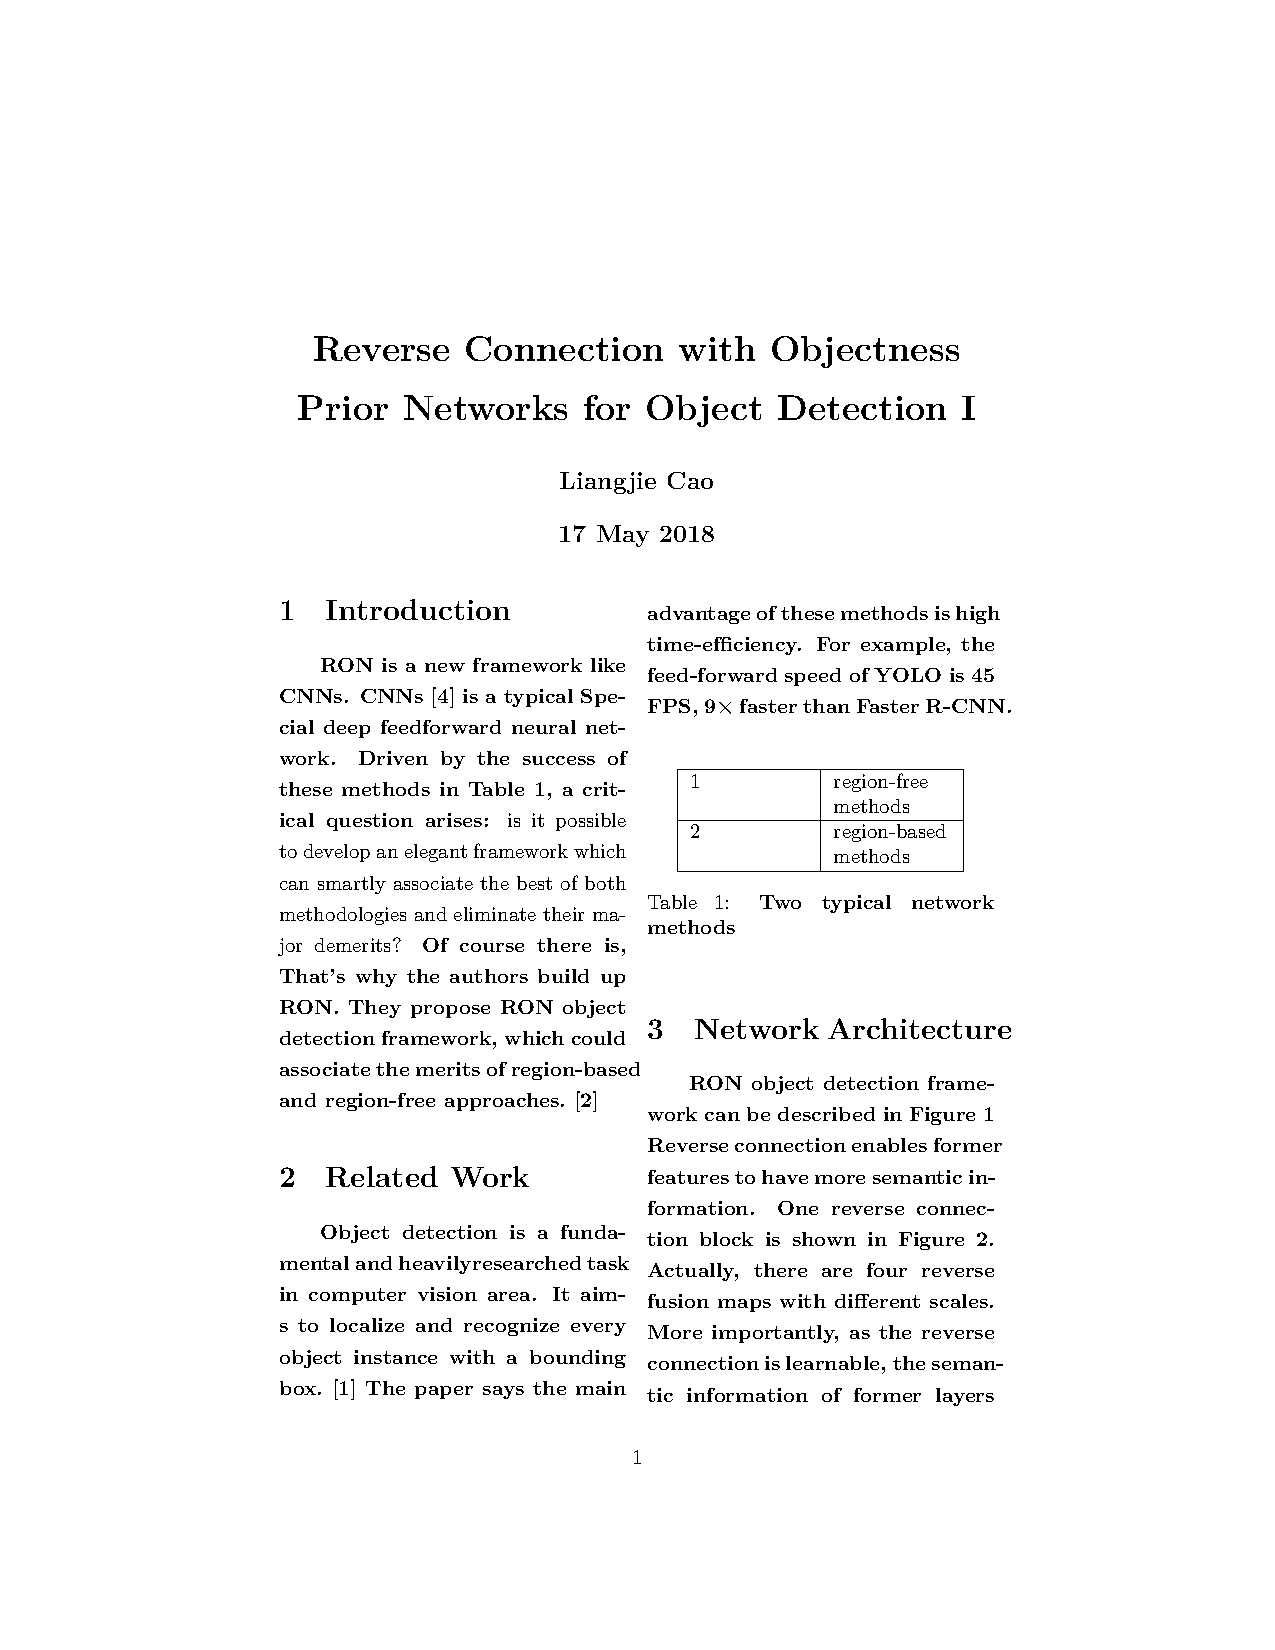
\includegraphics[width=0.5\textwidth]{RON.png}\\
 \caption{\textbf{RON object detection overview}}\label{Figure1}
 \end{figure}
\par
\section{PASCAL VOC 2012}
\textbf{Actually the results, as shown in Table~\ref{Table2}, demonstrate that our model performs the best on this dataset. Compared with Faster R-CNN and other variants\cite{name6}\cite{name7}, the proposed network is significantly better, mainly due to the reverse connection and the use of boxes from multiple feature maps. Compared with Faster R-CNN and other variants, the proposed network is significantly better, mainly due to the reverse connection and the use of boxes from multiple feature maps.
}
\begin{figure}[htbp]
  \centering
 \includegraphics[width=0.5\textwidth]{pro.png}\\
 \caption{\textbf{Recall versus number of proposals on the PASCAL VOC 2007 test set (with IoU = 0.5)}}\label{Figure2}
\end{figure}
\par
\section{MS COCO}
\textbf{To further validate the proposed framework on a larger and more challenging dataset, they conduct experiments on MS COCO  and report results from test-dev2015 evaluation server. Coco data set is a data set which can be used for image recognition + segmentation + capturing acquired by Microsoft team. With the standard COCO evaluation metric, Faster RCNN scores 21.9\% AP, and RON improves it to 27.4\% AP. Using the VOC overlap metric of IoU ≥0.5, RON384++ gives a 5.8 points boost compared with SSD500.\cite{name2}  It is also interesting to note that with 320×320 input size, RON gets 26.2\% AP, improving the SSD with 500×500 input size by 1.8 points on the strict COCO AP evaluation metric.
}\\
\section{From MS COCO to PASCAL VOC}
\textbf{As the categories on MS COCO are a superset of these on PASCAL VOC dataset, the fine-tuning process becomes easier compared with the ImageNet pretrained model. Starting from MS COCO pre-trained model, RON leads to 81.3\% mAP on PASCAL VOC 2007(Table~\ref{Table1}) and 80.7\% mAP on PASCAL VOC 2012.(Table~\ref{Table2} When submitting, the authors model with 384×384 input size has been ranked as the top 1 on the VOC 2012 leaderboard among VGG-16 based models. We note that other public methods with better results are all based on much deeper networks.  }
\section{Ablation Analysis}
\textbf{After removing the detection module, our network could get region proposals. We compare the proposal performance against Faster R-CNN\cite{name5} and evaluate recalls with different numbers of proposals on PASCAL VOC 2007 test set, as shown in Figure~\ref{Figure2}. Both Faster R-CNN and RON achieve promising region proposals when the region number is larger than 100. However, with fewer region proposals, the recall of RON boosts Faster R-CNN by a large margin. Specifically, with top 10 region proposals, these 320 model gets 80.7\% recall, outperforming Faster R-CNN by 20 points. This validates that our model is more effective in applications with less region proposals.
}
\section{Conclusion}
\textbf{They have presented RON, an efficient and effective object detection framework. We design the reverse connection to enable the network to detect objects on multi-levels of CNNs.On standard benchmarks, RON achieves state-of-the-art object detection performance. Maybe oneday I can do this professional work with my team.}
\onecolumn 
\begin{table}[!h]
 \begin{tabular}{p{1.5cm}|p{0.5cm}|p{0.5cm}p{0.5cm}p{0.5cm}p{0.5cm}p{0.5cm}p{0.5cm}p{0.5cm}p{0.5cm}p{0.5cm}p{0.5cm}p{0.5cm}p{0.5cm}p{0.5cm}p{0.5cm}p{0.5cm}p{0.5cm}p{0.5cm}p{0.5cm}p{0.5cm}p{0.5cm}}
    \hline
    Method & map & aero & bike & bird & boat & bottle & bus & car & cat & chair & cow & table & dog & horse & mbike & person & plant & sheep & sofa & train & tv \\
    \hline
    Fast R-CNN\cite{name1} & 70.0 & 77.0 & 78.1 & 69.3 & 59.4 & 38.3 & 81.6 & 78.6 & 86.7 & 42.8 & 78.8 & 68.9 & 84.7 & 82.0 & 76.6 & 69.9 & 31.8 & 70.1 & 74.8 & 80.4 & 70.4 \\
    Faster R-CNN\cite{name5} & 73.2 & 76.5 & 79.0 & 70.9 & 65.5 & 52.1 & 83.1 & 84.7 & 86.4 & 52.0 & \textbf{81.9} & 65.7 & 84.8 & 84.6 & 77.5 & 76.7 & 38.8 & 73.6 & 73.9 & 83.0 & 72.6 \\
    SSD300\cite{name4} & 72.1 & 75.2 & 79.8 & 70.5 & 62.5 & 41.3 & 81.1 & 80.8 & 86.4 & 51.5 & 74.3 & 72.3 & 83.5 & 84.6 & 80.6 & 74.5 & 46.0 & 71.4 & 73.8 & 83.0 & 69.1 \\
    SSD500\cite{name4} & 75.1 & 79.8 & 79.5 & 74.5 & 63.4 & 51.9 & 84.9 & \textbf{85.6} & 87.2 & 56.6 & 80.1 & 70.0 & 85.4 & 84.9 & 80.9 & 78.2 & 49.0 & \textbf{78.4} & 72.4 & 84.6  & 75.5   \\
    \hline
    RON320 & 74.2 & 75.7 & 79.4 & 74.8 & 66.1 & 53.2 & 83.7 & 83.6 & 85.8 & 55.8 & 79.5 & 69.5 & 84.5 & 81.7 & 83.1 & 76.1 & 49.2 & 73.8 & 75.2 & 80.3 & 72.5 \\
    RON384 & 75.4 & 78.0 & 82.4 & 76.7 & 67.1 & 56.9 & 85.3 & 84.3 & 86.1 & 55.5 & 80.6 & 71.4 & 84.7 & 84.8 & 82.4 & 76.2 & 47.9 & 75.3 & 74.1 & 83.8 & 74.5 \\
    RON320++ & 76.6 & 79.4 & \textbf{84.3} & 75.5 & 69.5 & 56.9 & 83.7 & 84.0 & 87.4 & 57.9 & 81.3 & 74.1 & 84.1 & 85.3 & 83.5 & 77.8 & 49.2 & 76.7 & 77.3 & 86.7 & 77.2 \\
    RON384++ & \textbf{77.6} & 86.0 & 82.5 & 76.9 & 69.1 & 59.2 & 86.2 & 85.5 & 87.2 & 59.9 & 81.4 & 73.3 & 85.9 & 86.8 & 82.2 & 79.6 & 52.4 & 78.2 & 76.0 & 86.2 & 78.0 \\
  \end{tabular}
  \caption{\textbf{Detection results on PASCAL VOC 2007 test set. The entries with the best APs for each object category are bold-faced.}} \label{Table1}
  \end{table} 
  \begin{table}[h]
 \begin{tabular}{p{1.5cm}|p{0.5cm}|p{0.5cm}p{0.5cm}p{0.5cm}p{0.5cm}p{0.5cm}p{0.5cm}p{0.5cm}p{0.5cm}p{0.5cm}p{0.5cm}p{0.5cm}p{0.5cm}p{0.5cm}p{0.5cm}p{0.5cm}p{0.5cm}p{0.5cm}p{0.5cm}p{0.5cm}p{0.5cm}}
    \hline
    Method & map & aero & bike & bird & boat & bottle & bus & car & cat & chair & cow & table & dog & horse & mbike & person & plant & sheep & sofa & train & tv \\
    \hline
    Fast R-CNN\cite{name1} & 68.4 & 82.3 & 78.4 & 70.8 & 52.3 & 38.7 & 77.8 & 71.6 & 89.3 & 44.2 & 73.0 & 55.0 & 87.5 & 80.5 & 80.8 & 72.0 & 35.1 & 68.3 & 65.7 & 80.4 & 64.2 \\
    OHEM\cite{name6} & 71.9 & 83.0 & 81.3 & 72.5 & 55.6 & 49.0 & 78.9 & 74.7 & 89.5 & 52.3 & 75.0 & 61.0 & \textbf{87.9} & 80.9 & 82.4 & 76.3 & 47.1 & 72.5 & 67.3 & 80.6 & \textbf{71.2}\\
    Faster R-CNN\cite{name5} 70.4 & 75.2 & 79.8 & 70.5 & 62.5 & 41.3 & 81.1 & 80.8 & 86.4 & 51.5 & 74.3 & 72.3 & 83.5 & 84.6 & 80.6 & 74.5 & 46.0 & 71.4 & 73.8 & 83.0 & 69.1 \\
    HyperNet\cite{name7} & 71.4 & 84.2 & 79.8 & 70.5 & 62.5 & 41.3 & 81.1 & 80.8 & 86.4 & 51.5 & 74.3 & 72.3 & 83.5 & 84.6 & 80.6 & 74.5 & 46.0 & 71.4 & 73.8 & 83.0 & 69.1 \\
    SSD300\cite{name4} & 70.3 & 84.2 & 76.3 & 69.6 & 53.2 & 40.8 & 78.5 & 73.6 & 88.0 & 50.5 & 73.5 & 61.7 & 85.8 & 80.6 & 81.2 & 77.5 & 44.3 & 73.2 & 66.7 & 81.1 & 65.8 \\
    SSD500\cite{name4} & 73.1 & 84.9 & 82.6 & 74.4 & 55.8 & 50.0 & 80.3 & 78.9 & 88.8 & 53.7 & 76.8 & 59.4 & 87.6 & 83.7 & 82.6 & 81.4 & 47.2 & 75.5 & 65.6 & 84.3  & 68.1   \\
    \hline
    RON320 & 71.7 & 84.1 & 78.1 & 71.0 & 56.8 & 46.9 & 79.0 & 74.7 & 87.5 & 52.5 & 75.9 & 60.2 & 84.8 & 79.9 & 82.9 & 78.6 & 47.0 & 75.7 & 66.9 & 82.6 & 68.4 \\
    RON384 & 73.0 & 85.4 & 80.6 & 71.9 & 56.3 & 49.8 & 80.6 & 76.8 & 88.2 & 53.6 & 78.1 & 60.4 & 86.4 & 81.5 & 83.8 & 79.4 & 48.6 & 77.4 & 67.7 & 83.4 & 69.5 \\
    RON320++ & 74.5 & \textbf{87.1} & 81.0 & 74.6 & 58.8 & 51.7 & 82.1 & 77.0 & 89.7 & 57.2 & 79.9 & 62.6 & 87.2 & 83.2 & 85.0 & 80.5 & 51.4 & 76.7 & 68.5 & 84.8 & 70.4\\
    RON384++ & 75.4 & 86.5 & 82.9 & 76.6 & 60.9 & 55.8 & 81.7 & 80.2 & 91.1 & 57.3 & 81.1 & 60.4 & 87.2 & 84.8 & 84.9 & 81.7 & 51.9 & 79.1 & 68.6 & 84.1 & 70.3 \\
  \end{tabular}
  \caption{\textbf{Results on PASCAL VOC 2012 test set. All methods are based on the pre-trained VGG-16 networks.}} \label{Table2}
  \end{table}
\twocolumn \bibliographystyle{plain}
\bibliography{yinyong1}
\end{document}

